% Section 2: The One-Bit Clock
%%%%%%%%%%%%%%%
\begin{en}
\newpage
 \tindex{1}{One-Bit Clock}%
 \ctindex{1}{Clock!One-Bit}{clock-one-bit}%
 \vspace{-\baselineskip}%
\btarget{sec:one-bit}\section{The One-Bit Clock}

Our first example is a clock.  We consider the simplest possible
clock: one that alternately shows the ``times'' 0 and 1.  Such a clock
controls the computer on which you are reading this, with its times
being displayed as the voltage on a wire.  A real clock should tick at
an approximately constant rate.  There is a lot to explain before we
can specify that requirement, so we are going to ignore it.  This
leaves a very simple computing device that just alternates between two
states: the state in which the clock displays 0 and the state in which
it displays~1.
\end{en}

\begin{ch}
\newpage
 \tindex{1}{One-Bit Clock}%
 \ctindex{1}{Clock!One-Bit}{clock-one-bit}%
 \vspace{-\baselineskip}%
\btarget{sec:one-bit}\section{单比特时钟}

我们考虑的第一个例子是一个尽可能简单的时钟:它交替显示``时间''0与1。
这类时钟控制着你正用于阅读本书的计算机,它的``时间''表现为电缆上的电压。
真实的时钟应该基本保持匀速行走。
我们忽略这种需求,因为如果要描述它,我们还需要解释很多事情。
% 要想描述这个需求,我们还需要解释很多事情,所以我们忽略它。
这样一来,我们只需要考虑一个在两种状态之间交替的非常简单的计算设备:
一个状态显示0,另一个状态显示1。
\end{ch}
%%%%%%%%%%%%%%%

%%%%%%%%%%%%%%%
\begin{en}
This may seem a strange example to choose because it has no
concurrency.  The clock does only one thing at a time.  A system can
do any number of things at a time.  \emph{One} is a simple special
case of \emph{any number}, and it's a good place to begin.  Learning
to specify sequential systems in \tlaplus\ teaches most of what you
need to know to specify concurrent systems.
\end{en}

\begin{ch}
  这似乎是个奇怪的例子,因为它不涉及并发。
  这个时钟一次只做一件事。
  在同一时刻,一个系统可以做任意多件事。
  \emph{一}是\emph{任意多}的简单的特殊情况,这是一个好的起点。
  学习使用 \tlaplus\ 描述顺序系统能让我们掌握描述并发系统所需的大多数知识。
\end{ch}
%%%%%%%%%%%%%%%


%%%%%%%%%%%%%%%
\begin{en}
\subsection{The Clock's Behaviors} \label{sec2.1}

We use the standard model to represent the clock.  This means that a
possible execution of the clock is represented by a 
  \tindex{2}{behavior}%
behavior, which is
a sequence of states, and a 
  \tindex{2}{state}%
state is an assignment of values to variables.  We model the clock
with a single variable $b$ that represents the clock ``face'', where
the assignment of 0 to $b$ represents the clock displaying 0, and the
assignment of 1 to $b$ represents its displaying 1.  We describe the
state that assigns the value 0 to $b$ by the formula $b=0$, and
similarly for $b=1$.
\end{en}

\begin{ch}
\subsection{时钟的行为} \label{sec2.1}

我们使用标准模型建模时钟。
也就是说,时钟的一次可能执行表示为一个%
  \tindex{2}{behavior}%
行为。
一个行为是一个状态序列,而一个%
  \tindex{2}{state}%
状态则是对变量的一种赋值。
我们用一个变量$b$表示``钟面'':
$b$赋值为0表示时钟显示0,赋值为1表示时钟显示1。
我们用公式$b=0$表示``变量$b$赋值为0''这一状态;$b=1$的含义类似。
\end{ch}
%%%%%%%%%%%%%%%

%%%%%%%%%%%%%%%
\begin{en}
If we start the clock displaying 0, then we can pictorially represent
its behavior as:
 \[ %\begin{equation} \label{eq1}
   b=0 \s{.701} -> \s{.701} b=1 \s{.701} -> \s{.701} b=0 
       \s{.701} -> \s{.701} b=1 \s{.701} -> \s{.701} \cdots
 \] %\end{equation}
where ``$\cdots$'' means that the clock goes on forever the same way.
Real clocks eventually stop; the best we can expect is that they keep
running for long enough.  However, it's more convenient to consider an
ideal clock that never stops, rather than having to decide for how
long we should require it to run.  So, we describe a clock
that runs forever.
\end{en}

\begin{ch}
  如果我们让时钟从0开始,那么它的行为可以形象地描述成:
  \[ %\begin{equation} \label{eq1}
    b=0 \s{.701} -> \s{.701} b=1 \s{.701} -> \s{.701} b=0 
        \s{.701} -> \s{.701} b=1 \s{.701} -> \s{.701} \cdots
  \] %\end{equation}
  其中,``$\cdots$''表示时钟永不停歇。
  真实的时钟总会停下来;我们只能期望它运行的时间足够长。
  但是,考虑一个理想的永不停歇的时钟更为方便,
  而不必决定它究竟需要运行多长时间。
  因此,我们描述一个永不停歇的时钟。
\end{ch}
%%%%%%%%%%%%%%%

%%%%%%%%%%%%%%%
\begin{en}
We could also let the clock start displaying 1, in which case
its behavior is
 \[ % \begin{equation} \label{eqclk1}
   b=1 \s{.701} -> \s{.701} b=0 \s{.701} -> \s{.701} b=1 
       \s{.701} -> \s{.701} b=0  \s{.701} -> \s{.701} \cdots
 \] % \end{equation}
These two are the only possible behaviors of the one-bit
clock.
\end{en}

\begin{ch}
  我们也可以让时钟从1开始,在这种情况下,它的行为如下所示:
  \[ % \begin{equation} \label{eqclk1}
    b=1 \s{.701} -> \s{.701} b=0 \s{.701} -> \s{.701} b=1 
        \s{.701} -> \s{.701} b=0  \s{.701} -> \s{.701} \cdots
  \] % \end{equation}
  以上行为是单比特时钟仅有的两种行为。
\end{ch}
%%%%%%%%%%%%%%%

\pause

%%%%%%%%%%%%%%%
\begin{en}
\noindent
%
Remember that, although I have been calling them behaviors of the
clock, what I have really described are the behaviors in the standard
model of an abstraction of a real clock.  The display of a clock moves
continuously from one value to the next.  In a digital clock, the
transition may be too fast for us to see the intermediate values; but
they are there.  We are specifying an abstraction of the clock in
which these continuous changes are represented by discrete steps
(state changes).
\end{en}

\begin{ch}
  需要记住的是,尽管我们一直在使用``时钟的行为''这一说法,
  实际上,我们所描述的是``真实时钟的某种抽象的标准模型的行为''。
  真实时钟的钟面从一个值连续地变换成下一个值。
  虽然,在数字时钟里,这种变换可能发生得太快,以至于我们看不到中间值,
  但是它们是客观存在的。
  在我们所描述的时钟抽象里,这种连续的变换被表示为离散的步骤(状态变化)。
\end{ch}
%%%%%%%%%%%%%%%

% It may seem strange to call the ticking of a clock a computation.  We
% usually think of a computation as something that stops after producing
% a result---perhaps the first million digits of $\pi$.  But by that
% definition, our computers do very little computing.  We use them
% mostly for reading email, listening to music, and other ongoing tasks.
% What our one-bit clock does is typical of today's computations; it's
% just a lot simpler.
% 
% The term \emph{computation} is not very descriptive of what today's
% digital devices do.  I will therefore abandon it and use
% \emph{behavior} instead.  A computing device is therefore specified by
% describing all its behaviors, where a behavior is a sequence of
% states.  A state is an assignment of values to some collection of
% variables.  For the simple clock, the collection consists of the
% single variable $b$.

%%%%%%%%%%%%%%%
\begin{en}
\subsection{Describing the Behaviors}
\xlabel{main:one-bit:describing}

To describe a computing device, we must describe all its possible
behaviors.  I was able to list all the possible behaviors of the
one-bit clock, but that isn't feasible for any but the simplest
computing devices.  Even displaying a single behavior of a complex
device would be hard, and most computing devices have too many
behaviors to list---often, infinitely many behaviors.
\end{en}

\begin{ch}
  \subsection{描述行为}
  \xlabel{main:one-bit:describing}
  要描述一个计算设备,需要描述它的所有可能行为。
  我能够枚举单比特时钟的所有可能行为,
  但是枚举对于稍显复杂的计算设备就不可行了。
  有时,仅仅是展示复杂计算设备的单个行为都是困难的,
  更何况大多数计算设备的行为多到不胜枚举——通常是无穷多的。
\end{ch}
%%%%%%%%%%%%%%%

%%%%%%%%%%%%%%%
\begin{en}
If we look beyond their syntax, we find that practical languages for
describing computing devices specify two things:
\begin{itemize}
\item The possible initial states.

\item The possible 
  \tindex{2}{step}%
steps.  (Remember that a step is a transition from one state to the
next.)
\end{itemize}
For example, here's how the one-bit clock might be
described in a (nonexistent) programming language.
\begin{program}
\kwd{variable} $b$: \s{-.6}0, 1; \V{.3}
\kwd{while} (\kwd{true}) \{ \kwd{if} ($b=0$) $b$ := 1 
                          \kwd{else} $b$ := 0; \} 
\end{program}
The first line says that the possible initial states are $b=0$ and
$b=1$.  The second line says that if $b$ equals 0, then in the next
state it equals 1; and if it equals 1, then in the next state it
equals~0.
\end{en}

\begin{ch}
  \fixme{跳出语法层面,我们发现,要描述计算设备,一门语言需要指明以下两点:}
  \begin{itemize}
    \item 所有可能的初始状态。
    \item 所有可能的%
	\tindex{2}{step}%
	步骤。(\emph{步}即状态转换。)
  \end{itemize}
  例如,使用某种(假想的)编程语言,单比特时钟可以描述如下:
  \begin{program}
  \kwd{variable} $b$: \s{-.6}0, 1; \V{.3}
  \kwd{while} (\kwd{true}) \{ \kwd{if} ($b=0$) $b$ := 1 
			    \kwd{else} $b$ := 0; \} 
  \end{program}
  第一行指明可能的初始状态是$b=0$或$b=1$。
  第二行指明如果$b$当前为0,那么在下一个状态$b$为1;
  如果$b$当前为1,那么在下一个状态$b$为0。
\end{ch}
%%%%%%%%%%%%%%%

%%%%%%%%%%%%%%%
\begin{en}
Instead of inventing a whole new language for describing initial
states and possible next states, we will do it with mathematics.  We
do this using the Boolean operators $\land$ and $\lor$.  If you are
not as familiar with these operators of simple logic as you are with
the operators $+$ and $-$ of arithmetic, you should
\target{andor}\textsf{\rref{math}{mathlogic}{detour to a discussion
of logic.}}.
\end{en}

\begin{ch}
  我们使用数学语言来描述初始状态与可能的后继状态,
  而不是发明一门全新的语言。
  我们使用布尔操作符 $\land$ 与 $\lor$。
  如果你不像熟悉算术操作符 $+$ 与 $-$ 那样熟悉这些简单的逻辑操作符,
  你应该%
  \target{andor}\textsf{\rref{math}{mathlogic}{先看一下``关于逻辑的一些讨论''}}.
\end{ch}
%%%%%%%%%%%%%%%

%%%%%%%%%%%%%%%
\begin{en}
Describing the initial states is simple; we just assert that the 
initial value of $b$ is 0 or 1.  This assertion is expressed by
the formula:
 \[ (b=0) \; \/ \; (b=1)\]
We call this formula the 
  \tindex{1}{initial predicate}%
  \ctindex{1}{predicate!initial}{predicate-initial}%
\emph{initial predicate}.
\end{en}

\begin{ch}
  初始状态易于描述。
  我们只需要断言 $b$ 的初始值是0或者1,用公式表示如下:
  \[ (b=0) \; \/ \; (b=1)\]
  我们称该公式为%
    \tindex{1}{initial predicate}%
    \ctindex{1}{predicate!initial}{predicate-initial}%
  \emph{\tlainitpredicate}。
\end{ch}
%%%%%%%%%%%%%%%

%%%%%%%%%%%%%%%
\begin{en}
To describe the possible steps, we have to write a mathematical
formula relating the values of $b$ in two states: the first state of
the step and its next state.  We do this by letting $b$ mean the
value of $b$ in the first state, and 
 \ctindex{1}{+2a@\mmath{'} (prime)}{+2a}%
 \ctindex{1}{prime (\mmath{'})!of a variable}{prime-variable}%
$b'$ mean its value in the next state.  There are two possible steps:
one with $b=0$ and $b'=1$, and the other with $b=1$ and $b'=0$.  Thus,
all possible steps are described by this formula:
 \[   ((b=0) \; /\ \; (b'=1)) \; \/ \; ((b=1) \; /\ \; (b'=0)) 
 \]
Even this tiny formula is a little hard to read because of all the
parentheses.  For larger formulas with conjunctions and disjunctions,
it can get almost impossible to keep track of the parentheses.
\tlaplus\ allows us to write conjunctions and disjunctions
as lists of formulas bulleted by $/\ $ or $\/ $.  We can therefore
also write this formula as%
\marginpar{We can also write the initial predicate as\\
             \s{1}$\begin{disj}
                   b=0 \\ b=1
                   \end{disj}$ \V{.4}\popref{junct-warning}{\bf Warning.}}
 \[ \begin{disj}
    (b=0) \; /\ \; (b'=1) \\ (b=1) \; /\ \; (b'=0)
    \end{disj}
   \s{2}\mbox{or} \s{2}
%
 \begin{disj}
    \begin{conj}
    b=0 \\ b'=1
    \end{conj} \\
    \begin{conj}
    b=1 \\ b'=0
    \end{conj}
    \end{disj}
 \] 
However it is written, we usually call this formula the
  \ctindex{1}{next-state action@next-state action\icmd{target}{next-state-target}}{next-state action}%
  \ctindex{1}{next-state relation|see{\icmd{lref}{next-state-target}{next-state action}}}{next-state-rel}%
  \ctindex{1}{action!next-state}{action-next-state}%
\emph{next-state action} or sometimes the \emph{next-state relation}.
\end{en}
\begin{ch}
  要描述可能的\tlastep{},我们必须使用一个数学公式将 $b$ 
  在两个状态——\fixme{该\tlastep{}的出发状态与后继状态}——中的值联系起来。
  我们使用 $b$ 表示 $b$ 在出发状态的值,%
    \ctindex{1}{+2a@\mmath{'} (prime)}{+2a}%
    \ctindex{1}{prime (\mmath{'})!of a variable}{prime-variable}%
  $b'$ 表示 $b$ 在后继状态的值。
  有两种可能的\tlastep{}:
  一种是 $b = 0$ 且 $b' = 1$;
  另一种是 $b = 1$ 且 $b' = 0$。
  因此,所有可能的\tlastep{}可用如下公式表示:
  \[   
    ((b=0) \; /\ \; (b'=1)) \; \/ \; ((b=1) \; /\ \; (b'=0)) 
  \]
  由于括号的原因,即使这么短的公式也有点难以阅读。
  对于由合取与析取构成的更长的公式,我们几乎无法追踪其中的括号。
  \tlaplus\ 允许我们将合取与析取写成标有符号 $/\ $ 或 $\/ $ 的公式列表。
  因此,上式也可以写成:%
  \marginpar{我们也可以将\tlainitpredicate{}写成:\\
               \s{1}$\begin{disj}
                     b=0 \\ b=1
                     \end{disj}$ \V{.4}\popref{junct-warning}{\bf 警告.}}
  \[ \begin{disj}
     (b=0) \; /\ \; (b'=1) \\ (b=1) \; /\ \; (b'=0)
     \end{disj}
    \s{2}\mbox{or} \s{2}
  %
  \begin{disj}
     \begin{conj}
     b=0 \\ b'=1
     \end{conj} \\
     \begin{conj}
     b=1 \\ b'=0
     \end{conj}
     \end{disj}
  \] 
  不管写成什么形式,我们通常将该公式称为%
  \emph{\tlanextstateaction},有时也称为\emph{\tlanextstaterelation}。
\end{ch}
%%%%%%%%%%%%%%%

% 1st
%%%%%%%%%%%%%%%
\begin{en}
\subsection{Writing the Specification}

Let's now turn the initial predicate and next-state action into a
\tlaplus\ specification.  
  \popref{open-new-spec}{Open a new spec}
in the 
  \tindex{1}{Toolbox}%
 \hyperref{http://research.microsoft.com/en-us/um/people/lamport/tla/toolbox.html}{}{}{\protect\tlaplus\
Toolbox}.
Name the specification and
its root module \emph{OneBitClock}.  This creates a new module file
named \texttt{OneBitClock.tla} and opens an editor on it.
\end{en}

\begin{ch}
  \subsection{编写规约}

  现在,我们将\tlainitpredicate{}与\tlanextstateaction{}写入 \tlaplus\ \tlaspec。
  在%
    \tindex{1}{Toolbox}%
  \hyperref{http://research.microsoft.com/en-us/um/people/lamport/tla/toolbox.html}{}{}{\protect\tlaplus\ \tlatoolbox}%
  里%
  \popref{open-new-spec}{打开新规约}。
  将\tlaspec{}与它的根\tlamodule{}命名为 \emph{OneBitClock}。
  这会创建一个名为 \texttt{OneBitClock.tla} 的\tlamodule{}文件,
  并打开一个编辑器。
\end{ch}
%%%%%%%%%%%%%%%

% 2nd
%%%%%%%%%%%%%%%
\begin{en}
The newly created module looks something like this in the editor:
\begin{display}
\begin{verbatim}
------------------- MODULE OneBitClock --------------------

===========================================================
\* Modification History
\* Created Mon Dec 13 09:57:04 PST 2010 by jones
\end{verbatim}
\end{display}
The first line is the 
 \tindex{1}{module opening}%
 \ctindex{1}{opening!of module}{opening-of-module}%
\emph{module opening}; the last line is the
 \tindex{1}{module closing}%
 \ctindex{1}{closing!of module}{closing-of-module}%
\emph{module closing}.  All text before the opening and after the
closing is not part of the module and is ignored.  Each sequence of
\verb|-| characters in the opening and the sequence of \verb|=|
characters in the closing can be of any length greater than~3.  
The opening and closing are printed as follows:
\begin{display}
\begin{module}{OneBitClock}
\mbox{\strut}
\end{module}
\end{display}
We now assign names to our initial predicate and next-state action.  I
have traditionally called them $Init$ and $Next$.  However, we will be
defining some alternative initial predicates and next-state relations,
so let's call these $Init1$ and $Next1$.  These formulas are defined
as follows.
\begin{display}
\begin{notla}
Init1 == (b=0) \/ (b=1)
     
Next1 == \/ /\ b = 0
            /\ b' = 1
         \/ /\ b = 1
            /\ b' = 0
\end{notla}
\begin{tlatex}
\@x{ Init1\@s{4.12} \.{\defeq} ( b \.{=} 0 ) \.{\lor}
   ( b \.{=} 1 )}\ascii{OneBitClock-1}\target{init1-next1-clock}%
\par\vspace{8.0pt}%
\@x{ Next1 \.{\defeq} \.{\lor} \.{\land} b \.{=} 0}%
  \target{main:next1}%
\@x{\@s{55.94} \.{\land} b' \.{=} 1}%
\@x{\@s{44.83} \.{\lor} \.{\land} b \.{=} 1}%
\marginpar[1]{Remember that you can click on the link to the
 \textsc{ascii} version and copy the text.}%
\@x{\@s{55.94} \.{\land} b' \.{=} 0}%
\end{tlatex}
\end{display}
These two \tlaplus\ statements define $Init1$ and $Next1$ to be the
two formulas.  Thus, anywhere in the spec following the definition of
$Init1$, typing $Init1$ is completely equivalent to typing
\tlabox{((b=0)\/(b=1))}.  The symbol $\!==\!$ (typed \verb|==|) is
read \emph{is defined to equal}.
\end{en}

\begin{ch}
  编辑器中新模块的内容如下所示:
  \begin{display}
  \begin{verbatim}
  ------------------- MODULE OneBitClock --------------------

  ===========================================================
  \* Modification History
  \* Created Mon Dec 13 09:57:04 PST 2010 by jones
  \end{verbatim}
  \end{display}
  第一行是%
    \tindex{1}{module opening}%
    \ctindex{1}{opening!of module}{opening-of-module}%
  \emph{\tlamoduleopening}语句,
  最后一行是%
    \tindex{1}{module closing}%
    \ctindex{1}{closing!of module}{closing-of-module}%
  \emph{\tlamoduleclosing}语句。
  \tlamoduleopening{}语句之前以及\tlamoduleclosing{}语句之后的内容
  都不属于模块,会被忽略。
  \tlamoduleopening{}语句中每个 \verb|-| 序列
  与\tlamoduleclosing{}语句中的 \verb|=| 序列的长度可以是大于3的任意值。
  \tlamoduleopening{}与\tlamoduleclosing{}显示如下:
  \begin{display}
    \begin{module}{OneBitClock}
    \mbox{\strut}
    \end{module}
  \end{display}
  现在,我们为上面定义的\tlainitpredicate{}与\tlanextstateaction{}命名。
  习惯上,我称它们为 $Init$ 与 $Next$。
  不过,由于后面我们会给出几种不同的定义,
  所以目前我们称之为 $Init1$ 与 $Next1$,定义如下:
  \begin{display}
    \begin{notla}
    Init1 == (b=0) \/ (b=1)
	 
    Next1 == \/ /\ b = 0
		/\ b' = 1
	     \/ /\ b = 1
		/\ b' = 0
    \end{notla}
    \begin{tlatex}
    \@x{ Init1\@s{4.12} \.{\defeq} ( b \.{=} 0 ) \.{\lor}
       ( b \.{=} 1 )}\ascii{OneBitClock-1}\target{init1-next1-clock}%
    \par\vspace{8.0pt}%
    \@x{ Next1 \.{\defeq} \.{\lor} \.{\land} b \.{=} 0}%
      \target{main:next1}%
    \@x{\@s{55.94} \.{\land} b' \.{=} 1}%
    \@x{\@s{44.83} \.{\lor} \.{\land} b \.{=} 1}%
    \marginpar[1]{你可以点击上面的链接,查看并拷贝公式的 \textsc{ascii} 版本。}%
    \@x{\@s{55.94} \.{\land} b' \.{=} 0}%
    \end{tlatex}
  \end{display}
  上面两个 \tlaplus\ 语句分别将 $Init1$ 和 $Next1$ 定义为一个公式。
  因此,在 $Init1$ 定义语句之后的任何地方,
  $Init1$ 都完全等价于 \tlabox{((b=0)\/(b=1))}。
  符号 $\!==\!$(输入\verb|==|)读作``\emph{\tladefeq}''。
\end{ch}
%%%%%%%%%%%%%%%

% 3rd
%%%%%%%%%%%%%%%
\begin{en}
Now \popref{save-module}{save the module}, which should cause the
Toolbox to parse the module.  (If it doesn't, go to the
\popref{parser-preferences}{TLA+ Parser Preferences menu}.)  The
parser will report six errors, all complaining that $b$ is an unknown
operator.  Clicking on each error message in the \textsf{Parsing
Errors} view highlights the location of the error---in this case, the
location of the particular occurrence of $b$ that it is complaining
about.
\end{en}

\begin{ch}
  \popref{save-module}{保存模块},\tlatoolbox{}将自动解析。
  (否则,请查看\popref{parser-preferences}{TLA+ \tlaparser{}配置菜单}。)
  \tlaparser{}将报告六个错误,都在抱怨``$b$是一个未知的操作符''。
  点击\textsf{\tlaparsererror} 视图中的某条错误信息,将高亮显示该错误的位置,
  也就是 $b$ 的某次特定出现。
\end{ch}
%%%%%%%%%%%%%%%

%%%%%%%%%%%%%%%
\begin{en}
Every symbol that appears in the module must either be a
primitive \tlaplus\ operator or else defined or declared before its
first use.  We must 
  \ctindex{1}%
   {variable declaration (tla)@variable declaration (\icmd{tlaplus})}%
   {tla-var-decl}%
  \ctindex{1}{declaration!tla variable@\icmd{tlaplus} variable}%
   {var-decl-tla}%
declare $b$ to be a variable, which we do by
inserting the following declaration at the beginning of the module,
before the definitions of $Init1$.%
    \ctindex{1}{variable@\icmd{textsc}{variable}}{variable}%
\begin{display}
\begin{twocols}
$\VARIABLE b$ %\ascii{OneBitClock-2} 
\midcol \verb|VARIABLE b|
\end{twocols}
\end{display}
Saving \marginpar{The
\raisebox{-2pt}{\scalebox{.75}{
\includegraphics{parsed-icon.jpg}}}
 icon in the lower-right corner tells you
 that the spec has no parsing errors.}
will make the errors go away.
\end{en}

\begin{ch}
  模块中的每个符号都要么是一个原子 \tlaplus\ 操作符,
  \fixme{要么在使用前已被定义过或声明过}。
  我们需要
    \ctindex{1}%
     {variable declaration (tla)@variable declaration (\icmd{tlaplus})}%
     {tla-var-decl}%
    \ctindex{1}{declaration!tla variable@\icmd{tlaplus} variable}%
     {var-decl-tla}%
  声明 $b$ 是一个变量。
  具体做法是在 $Init1$ 定义语句之前插入如下声明语句:%
    \ctindex{1}{variable@\icmd{textsc}{variable}}{variable}%
  \begin{display}
  \begin{twocols}
  $\VARIABLE b$ %\ascii{OneBitClock-2} 
  \midcol \verb|VARIABLE b|
  \end{twocols}
  \end{display}
  保存模块,%
    \marginpar{右下角的%
    \raisebox{-2pt}{\scalebox{.75}{
\includegraphics{parsed-icon.jpg}}}
     图标表明该规约没有解析错误。}
  错误将自行消失。
\end{ch}
%%%%%%%%%%%%%%%

\pause
%
\noindent
%
%%%%%%%%%%%%%%%
\begin{en}
When talking about the 
  \target{two-meanings-of-spec}%
  \ctindex{1}{specification!two meanings of}{spec-two-meanings}%
\emph{specification} of the one-bit clock, we
can mean one of two things:
\begin{itemize}
\item The complete module.  

\item The initial predicate and next-state relation.
\end{itemize}
It is usually clear from the context which is meant.  To avoid
confusion, we can talk about the module rather than the specification
when we mean the first.  We use the term
  \tindex{1}{behavior specification}%
  \ctindex{1}{specification!behavior}{spec-behavior}%
\emph{behavior specification} to mean the second.
\end{en}

\begin{ch}
  当我们谈论单比特时钟的%
  \emph{\tlaspec}时,我们指的是
  \begin{itemize}
    \item 整个模块,或者
    \item \tlainitpredicate{}与\tlanextstaterelation{}。
  \end{itemize}
  我们通常可以依靠上下文分辨出具体指代的是什么。
  为了避免混淆,当我们\fixme{意指前者时},我们只谈论模块,而不谈规约。
  另外,我们使用术语%
    \tindex{1}{behavior specification}%
    \ctindex{1}{specification!behavior}{spec-behavior}%
  \emph{\tlabehaviorspec}指代后者。
\end{ch}
%%%%%%%%%%%%%%%

% 1st
%%%%%%%%%%%%%%%
\begin{en}
  \tindex{1}{pretty printing}%
  \vspace{-\baselineskip}%
\btarget{pretty-printing}\subsection{The Pretty-Printed Version of Your Spec}

In addition to the \textsc{ascii} version of the module that you edit,
the Toolbox can display a ``pretty-printed'' version.  This requires
the 
  \ctindex{1}{pdflatex@\icmd{texttt}{pdflatex}}{pdflatex}%
\texttt{pdflatex} program to be installed on your computer.
Information on doing that and on configuring the Toolbox's
pretty-printing options can be found in 
\marginpar{\rref{help}{toolbox-help}{How to find help pages in
                                     the Toolbox.}}
\helppage{spec/pretty-printing}{the relevant Toolbox help page}.
\end{en}

\begin{ch}
  \tindex{1}{pretty printing}%
  \vspace{-\baselineskip}%
  \btarget{pretty-printing}\subsection{\tlaprettyprinted{}规约}

  除了我们所编辑的 \textsc{ascii} 版本的模块,
  \tlatoolbox{}还可以显示一种``\tlaprettyprinted{}''版本。
  这需要安装
    \ctindex{1}{pdflatex@\icmd{texttt}{pdflatex}}{pdflatex}%
  \texttt{pdflatex} 程序。
  关于如何安装 \texttt{pdflatex},
  以及如何配置\tlatoolbox{}的``\tlaprettyprinting{}''选项,
  请参考%
  \marginpar{\rref{help}{toolbox-help}{如何找到\tlatoolbox{}的帮助页面。}}
  \helppage{spec/pretty-printing}{\tlatoolbox{}的相关帮助页面}。
\end{ch}
%%%%%%%%%%%%%%%

% 2nd
%%%%%%%%%%%%%%%
\begin{en}
To produce a pretty-printed version of the module, click on the
\textsf{File} menu and choose \textsf{Produce PDF Version}.  The 
pretty-printed version will be displayed in a separate window within
the Toolbox, with \tlaplus\ expressions shown approximately the way
they are printed in this hyperbook.  You can switch
 \marginpar{\popref{pretty-printing-bug}{Does it do something else?}}
between the \textsc{ascii} and
pretty-printed versions by clicking either the \textsf{TLA Module} or
\textsf{PDF Viewer} tab in the top-left corner of the module's window.
Editing the \textsc{ascii} version does not automatically change the
pretty-printed version.  You need to run the
\textsf{File}\,/\,\textsf{Produce PDF Version} command again to update it.
\end{en}

\begin{ch}
  要生成模块的\tlaprettyprinting{}版本,
  请点击 \tlafilemenu{} 菜单,选择 \tlaproducepdfmenu{}。
  生成的\tlaprettyprinting{}版本将显示在工具箱的一个单独的窗口中,
  其中的 \tlaplus\ \fixme{表达式的显示方式与本书所展示的差不多}。
  你可以通过点击模块窗口左上角的 \tlamoduletab{} 或者 \tlapdfviewertab{} 标签
  在 \textsc{ascii} 版本与\tlaprettyprinting{}版本之间进行切换。
  编辑 \textsc{ascii} 版本并不会自动更新\tlaprettyprinting{}版本,
  你需要再次运行 \tlafilemenu{}\,/\,\tlaproducepdfmenu{} 命令。
  % 以更新\tlaprettyprinting{}版本。
\end{ch}
%%%%%%%%%%%%%%%

% 3rd
%%%%%%%%%%%%%%%
\begin{en}
The pretty-printed version is produced in a file
\texttt{OneBitClock.pdf} that the Toolbox puts in the same directory
as the module file \texttt{OneBitClock.tla}.  You can print that file
to get a paper version.
\end{en}

\begin{ch}
  \tlaprettyprinting{}版本的文件名是 \texttt{OneBitClock.pdf},
  与模块文件 \texttt{OneBitClock.tla} 存放在同一个文件夹下。
  你可以把它\fixme{打印成纸质版本}。% 打印出来?
\end{ch}
%%%%%%%%%%%%%%%

% 1st
%%%%%%%%%%%%%%%
\begin{en}
\subsection{Checking the Specification}

Let's now get the 
  \tindex{1}{TLC}%
TLC model checker to check this specification.
\popref{create-new-model}{Create a new model}.  This opens a 
  \ctindex{1}{model!editor}{model-editor}% 
model editor on the model.  That editor has three pages; the model is
opened to the \textsf{Model Overview} page.
\end{en}

\begin{ch}
  \subsection{验证规约}

  现在,我们使用 
    \tindex{1}{TLC}%
  TLC \tlcmodelchecker{}来验证该规约。
  \popref{create-new-model}{创建一个新的模型}。
  这将打开一个包含三个页面的%
    \ctindex{1}{model!editor}{model-editor}% 
  模型编辑器,\fixme{默认打开的}是 \tlcmodeloverview{}页面。
\end{ch}
%%%%%%%%%%%%%%%

% 2nd
%%%%%%%%%%%%%%%
\begin{en}
Enter $Init1$ and $Next1$ in the appropriate fields as the initial
predicate and next-state relation, and \popref{run-tlc}{run TLC}\@.
TLC runs for a couple of seconds and stops, reporting no errors.  This
means that the specification is sensible.  More precisely, it means
that our specification completely determines a collection of
behaviors.
\end{en}

\begin{ch}
  将\tlainitpredicate{} $Init1$ 与\tlanextstaterelation{} $Next1$ 填入
  相应的文本域,并\popref{run-tlc}{运行 \tlc{}}\@。
  \tlc{}将在几秒钟后停下来,并且没有发现错误。
  这意味着该规约是合理的,更准确地说,它完全确定了一组行为。
\end{ch}
%%%%%%%%%%%%%%%

\pause

% 3rd
%%%%%%%%%%%%%%%
\begin{en}
\noindent
%
Let's change the specification so it doesn't determine a collection of
behaviors.  Go to the module editor (by clicking on its tab) and
modify the definition of $Next1$ by replacing \verb|/\ b' = 0| with
\verb|/\ b' = "xyz"|.  The second disjunct allows a step starting with
$b=0$ to set $b$ (change its value) to the
\rref{math}{strings}{string} \tlastring{xyz}.  Save the module, return
to the model editor, and run TLC again.  This time it reports the
error:
\begin{widedisplay}\small \tt
Attempted to check equality of string "xyz" with non-string: 0
\end{widedisplay}
The \textsf{TLC Errors} window also shows:%
 \marginpar{You can \popref{resize-errors-view}{resize the fields of the 
\textsf{TLC Errors} view}.}
\begin{display}
\scalebox{.75}{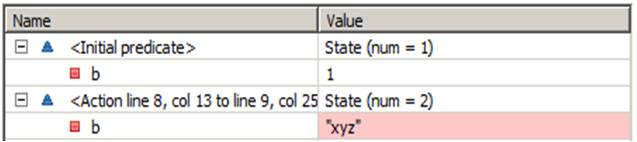
\includegraphics{OneBitClock-errortrace-1.jpg}}
\end{display}
This describes the following error trace: 
 \[ b=1 \s{.701} -> \s{.701} b = "xyz"
 \]
The trace is the beginning of a behavior that TLC was constructing
when it encountered an error.  The light-red background for the value
$"xyz"$ of $b$ indicates that it is different from the value of $b$ in
the previous state.  Double click on this line of the error trace:
\begin{display}
\scalebox{.75}{
\includegraphics{OneBitClock-errortrace-2.jpg}}
\end{display}
This raises the module editor, showing in part:
\begin{display}
\scalebox{.75}{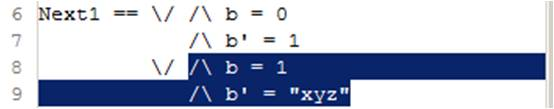
\includegraphics{OneBitClock-1.jpg}}
\end{display}
The highlighted portion is the disjunct of the next-state action $Next1$
that permits the step \,\tlabox{b=1 \, -> \, b = "xyz"}\,.
\end{en}

\begin{ch}
  \noindent
  %
  让我们修改规约,以使得它不能确定一组行为。
  切换到模块编辑器(可点击相应标签页),
  将 $Next1$ 定义中的 \verb|/\ b' = 0| 修改为 \verb|/\ b' = "xyz"|。
  现在,$Next1$ 的第二个析取式允许\fixme{一个\tlastep{}将 $b$ 从数字 0 设置为}
  \rref{math}{strings}{字符串} \tlastring{xyz}。
  保存模块,回到模型编辑器,再次运行 \tlc{}。
  这次,\tlc{} 将报告如下错误:
  \begin{widedisplay}\small \tt
    Attempted to check equality of string "xyz" with non-string: 0 \\
    (试图检查字符串 "xyz" 与非字符串 0 的相等性)
  \end{widedisplay}
  \tlcerrors{} 窗口如下所示:%
    \marginpar{你可以 \popref{resize-errors-view}{调整 \tlcerrors{} 视图中文本域的大小。}}
  \begin{display}
    \scalebox{.75}{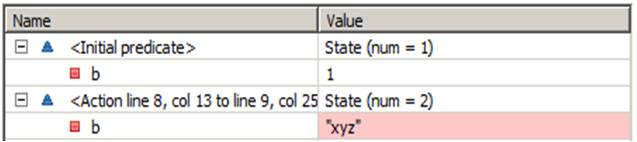
\includegraphics{OneBitClock-errortrace-1.jpg}}
  \end{display}
  它描述了一条\fixme{\tlcerrortrace{}}:
  \[ 
    b=1 \s{.701} -> \s{.701} b = "xyz"
  \]
  这是 \tlc{} 在遇到错误之前\fixme{所构造的行为的开头部分}。
  变量 $b$ 的值 $"xyz"$ 带有淡红色背景,
  这表示该值与前一个状态中 $b$ 的取值不同。
  双击\tlcerrortrace{}中的如下一行,
  \begin{display}
    \scalebox{.75}{
\includegraphics{OneBitClock-errortrace-2.jpg}}
  \end{display}
  将\fixme{跳转到模块编辑器的如下部分}:
  \begin{display}
    \scalebox{.75}{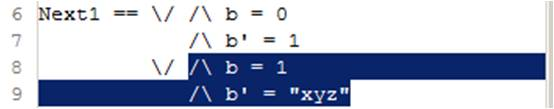
\includegraphics{OneBitClock-1.jpg}}
  \end{display}
  高亮显示的部分是\tlanextstateaction{} $Next1$ 中
  允许 \,\tlabox{b=1 \, -> \, b = "xyz"}\, \tlastep{}的析取式。
\end{ch}
%%%%%%%%%%%%%%%

% 4th
%%%%%%%%%%%%%%%
\begin{en}
To calculate the possible next states from the state with $b="xyz"$,
TLC had to compute the value of the formula $"xyz"=0$.  (The rest of
the error message tells you that it was computing that formula in
order to evaluate the subformula $b=0$ of the definition of $Next1$.)
TLC couldn't do that because the semantics of \tlaplus\ do not
determine whether or not a string is equal to a 
  \marginpar{\popref{strings-vs-numbers}{Why shouldn't 
  \tlastring{xyz} be unequal
   to $0$?}}
number.  It could
therefore not determine if the formula $"xyz"=0$ equals \TRUE\ or
\FALSE, so it reported an error. 
\end{en}

\begin{ch}
  要计算满足 $b="xyz"$ 的状态 \fixme{with} 的所有可能的后继状态,
  \tlc{} 需要计算公式 $"xyz"=0$ 的值。
  (错误信息的剩余部分表明 \tlc{} 正在计算该公式,
  以便决定定义 $Next1$ 中的子公式 $b=0$ 的真假。)
  \tlc{} 无法完成该工作,
  因为 \tlaplus\ 的语义没有指明一个字符串是否等于一个
    \marginpar{\popref{strings-vs-numbers}{\fixme{Why shouldn't 
      \tlastring{xyz} be unequal to $0$?}}}
  数字。
  所以,\tlc{} 无法确定公式 $"xyz"=0$ 的值是 \TRUE\ 还是 \FALSE,
  因此它报告了一个错误。
\end{ch}
%%%%%%%%%%%%%%%

% 5th
%%%%%%%%%%%%%%%
Restore the original definition of $Next1$ by replacing $"xyz"$ with 0
and save the module.  Go back to the model editor and run TLC again.
It should once again find no error.

\begin{ch}
\end{ch}
%%%%%%%%%%%%%%%

\pause
%
\noindent 
%
In the \textsf{Statistics} section of the \textsf{Model Checking
Results} page, the \textsf{State space progress} table tells you that
TLC found 2 distinct states.  The diameter of 1 means that 1 is the
largest number of steps (transitions from one state to the next) that
an execution of the one-bit clock can take before it repeats a state.

The one-bit clock is so simple there isn't much to check.  But there
is one property that we can and should check of just about any spec:
that it is 
  \tindex{1}{type correctness}%
``type correct''.  Type correctness of a \tlaplus\ specification
means that in every state of every behavior allowed by the spec, the
value of each variable is in the set of values that we expect it to
have.  For the one-bit clock, we expect the value of $b$ always to be
either 0 or 1.  This means that we expect the formula $b\in\{0,1\}$ to
be true in every state of every behavior of $b$.  If you are the least
bit unsure of what this formula means,
\target{sets}\textsf{\rref{math}{sets-intro}{detour to an introduction
to sets}}.\xlabel{main:simple-sets-return}

A formula that is true in all states of all behaviors allowed by a
spec is called an 
 \tindex{1}{invariant}%
\emph{invariant} of the spec.  Go to the
\textsf{Invariants} subsection of the \textsf{What to Check} section
of the model editor's\marginpar[.5]{Use the tabs at the top of the model
editor view to select the page.} \textsf{Model Overview} page.  Open
that subsection (by clicking on the {\bf \textsf{+}}), click on
\textsf{Add}, and enter the following formula:%
\begin{display}
\begin{twocols}
$b \in \{0, 1\}$
\midcol
\verb|b \in {0, 1}|
\end{twocols}
\end{display}
(Note that $\in$ is typed \verb|\in|.)  Click on \textsf{Finish}, and
then run TLC again on the model.  TLC should find no errors,
indicating that this formula is an invariant of the spec.

Because \tlaplus\ has no types, it has no type declarations.  As this
spec shows, there is no need for type declarations.  We don't need to
declare that $b$ is of type $\{0,1\}$ because that's implied by the
specification.  However, the reader of the spec doesn't discover that
until after she has read the definitions of the initial predicate and
next-state action.  In most real specifications, it's hard to
understand those definitions without knowing what the set of possible
values of each variable is.  It's a good idea to give the reader that
information by defining the 
 \ctindex{1}{invariant!type correctness}{inv-type-correct}%
 \ctindex{1}{type correctness!invariant}{type-correct-inv}%
type-correctness invariant in the spec,
right after the declaration of the variables.  So, let's add the
following definition to our spec, right after the declaration of $b$.
\begin{display}
\begin{twocols}
$TypeOK == b \in \{0,\,1\}$
\midcol
\verb|TypeOK == b \in {0,1}|
\end{twocols}
\end{display}
Save the spec and let's tidy up the model by using $TypeOK$ rather
than \tlabox{b \in \{0,\,1\}} as the invariant.  Go to the model
editor's \textsf{Model Overview} page, select the invariant you just
entered by clicking on it and hit \textsf{Edit} (or simply double-click on
the invariant), and replace the formula by \texttt{TypeOK}\@.  Click on
\textsf{Finish} and run TLC to check that you haven't made a mistake.

  \ctindex{1}{behavior!computing}{behavior-computing}%\
  \vspace{-\baselineskip}%
\subsection{Computing the Behaviors from the Specification}
\xlabel{sec:computing-clock-behaviors}

TLC checked that $TypeOK$ is an invariant of the specification of
the one-bit clock, meaning that it is true in all states of all
behaviors satisfying the specification.  TLC did this by computing
all possible behaviors that satisfy the initial predicate $Init1$ and
the next-state action $Next1$.  To understand how it does this, let's
see how we can do it.

We begin by computing one possible behavior.  A behavior is a sequence
of states.  To satisfy
the spec, the behavior's first state must satisfy the initial predicate
$Init1$.
A state is an assignment of values to all the spec's
variables, and this spec has only the single variable~$b$.  So to determine
a possible initial state, we must find an assignment of values to the
variable $b$ that satisfy $Init1$.  Since $Init1$ is defined to equal
 \[ (b=0) \/ (b=1) \]
there are obviously two such assignments: letting $b$ equal 0 or
letting it equal~1.  To construct one possible behavior satisfying the
spec, let's arbitrarily choose the starting state in which $b$
equals~1.  As before, we write that state as the formula $b=1$.

We next find a possible second state of the behavior.  For a behavior
to satisfy the spec, every pair of successive states must satisfy the
next-state action $Next1$, where the values of the unprimed variables
are the values assigned to them by the first state of the pair and the
values of the primed variables are the values assigned to them by the
second state of the pair.  The first state of our behavior is $b=1$.
To obtain the second state, we need to find a value for $b'$ that
satisfies $Next1$ when $b$ has the value 1.  We then let $b$ equal
that value in the second state.  To find this value, we substitute
$1$ for $b$ in $Next1$ and simplify the formula.  Recall that $Next1$
is defined to equal
 \[ \begin{disj}
    \begin{conj}
            b = 0 \\
            b' = 1
     \end{conj} \\
      \begin{conj}
         b = 1 \\
         b' = 0
     \end{conj}
    \end{disj}
 \]
We substitute 1 for $b$ and simplify as follows.
\begin{display}
\begin{tabbing}
   $\begin{disj}
    \begin{conj}
            1 = 0 \\
            b' = 1
     \end{conj} \\
      \begin{conj}
         1 = 1 \\
         b' = 0\vs{.75}
     \end{conj}
    \end{disj}$  \s{3} \=
    the formula obtained by substituting 1 for $b$ in $Next1$.\\
   $\mbox{} = \;\; \begin{disj}
    \begin{conj}
            \FALSE \\
            b' = 1
     \end{conj} \\
      \begin{conj}
         \TRUE \\
         b' = 0\vs{.75}
     \end{conj}
    \end{disj}$ \> because $\;(0=1) = \FALSE\;$ and $\;(1=1) = \TRUE$ \\
%
   $\mbox{} = \;\; \begin{disj}
         \FALSE    \\ b' = 0 
         \vs{.75}
    \end{disj}$ \> \begin{minipage}[t]{.75\textwidth}
                   because $\;\FALSE /\ F = \FALSE\;$ and 
                           $\;\TRUE /\ F = F\;$ \\
                   for any truth value $F$
                   \end{minipage} \\
%
   $\mbox{} = \;\; b'=0$ \> \begin{minipage}[t]{.6\textwidth}
                   because $\FALSE \/ F = F$ 
                   for any truth value $F$.
                   \end{minipage}
\end{tabbing}
\end{display}
This computation shows that if we substitute $1$ for $b$ in $Next1$,
then the only value we can then substitute for $b'$ that makes $Next1$
true is~0.  Hence, the second state of our behavior can only be $b=0$,
and our behavior starts with
 \[ b=1 \s{.701} -> \s{.701} b=0 \]
To find the third state of our behavior, we substitute $0$ for $b$ in
$Next1$ and find a value for $b'$ that makes $Next1$ true.  It should be
clear that the same type of calculation we just did shows that the only
possible value for $b'$ that makes $Next1$ true is~1.  (If it's not
clear, go ahead and do the calculation.)  The first three states
of our behavior therefore must be
 \[ b=1 \s{.701} -> \s{.701} b=0 \s{.701}-> \s{.701}  b=1
  \]
We could continue our calculations to find the fourth state of the
behavior, but we don't have to.  We've already seen that the only
possible state that can follow $b=1$ is $b=0$.  We can deduce
that \popref{finite-behaviors}{we must obtain the infinite behavior} 
 \[ b=1 \s{.701} -> \s{.701} b=0 \s{.701}-> \s{.701}  b=1 \s{.701} -> 
    \s{.701} b=0 \s{.701}-> \s{.701} \cdots
  \]
To find all possible behaviors, recall that the only other possible
starting state is $b=0$.  From the calculations we've already done,
we know that the only state that can follow $b=0$ is $b=1$.  We
therefore see that the only other possible behavior is
 \[ b=0 \s{.701}-> \s{.701}  b=1 \s{.701} -> \s{.701} b=0 \s{.701}-> \s{.701}  
    b=1 \s{.701} -> \s{.701} \cdots
  \]

\medskip

This example shows how we can compute all possible behaviors allowed
by a specification.  We construct as follows a
  \popref{directed-graph}{directed graph} 
$\mathcal{G}$, called the
  \ctindex{1}{graph!state}{graph-state}%
  \tindex{1}{state graph}%
  \target{main:state-graph}%
  \emph{state graph},
whose nodes are states:
\begin{enumerate}
\item We start by setting $\mathcal{G}$ to the set of all possible
initial states of behaviors, which we find by computing all possible
assignments of values to variables that make the initial predicate
true.

\item For every state $s$ in $\mathcal{G}$, we compute as follows all
possible states $t$ such that $s->t$ can be a step in a behavior.  We
substitute the values assigned to variables by $s$ for the unprimed
variables in the next-state action, and then compute all possible
assignments of values to the primed variables that make the next-state
action true.

\item For every state $t$ found in step 2: (i)~we add $t$ to $\mathcal{G}$
if it is not already in $\mathcal{G}$, and (ii)~we draw an edge from
$s$ to $t$.

\item We repeat steps 2 and 3 until no new states or edges can be
added to $\mathcal{G}$.
\end{enumerate}
If and when this process terminates, the nodes of $\mathcal{G}$
consist of all the 
  \tindex{1}{reachable state}%
  \ctindex{1}{state!reachable}{state-reachable}%
reachable states of the specifications---that is, all states that
occur in some behavior satisfying the specification.  Every behavior
satisfying the specification can be found by starting in an initial
state (found in step~1) and following a (possibly infinite) path in
$\mathcal{G}$.

\medskip

This procedure is used by TLC to compute all possible behaviors.  The
  \tindex{1}{state space progress table}%
\emph{State space progress} table in the \textsf{Statistics} section
of the \textsf{Model Checking Results} page gives the following
information about the graph $\mathcal{G}$ that it is constructing.
\begin{description}
\item[Diameter] The number of states in the longest path of
                $\mathcal{G}$ in which no state appears twice.
\item[States Found] The total number of (not necessarily distinct)
states it examined in step~1 or as successor states $t$ in step~2.

\item[Distinct States] The number of states that form the set of nodes
of $\mathcal{G}$.

\item[Queue Size] The number of states $s$ in $\mathcal{G}$ for which
step~2 has not yet been performed.
\end{description}
Of course, if the specification has an infinite number of reachable
states, this procedure will continue until $\mathcal{G}$ becomes so
large that TLC runs out of space.  However, this could take many years
because TLC keeps $\mathcal{G}$ and its queue of unexamined states on
disk when there is not enough room for them in memory.

Although TLC computes the behaviors that satisfy a specification the
same way we do, it's not nearly as smart as we are.  For example,
writing $1=b$ instead of $b=1$ in the initial predicate would make no
difference to us.  See how TLC reacts by making this change to the
definition of $Init1$ in module $OneBitClock$ and running TLC on the
model you created.  You will find that it produces the following error
report:
\begin{widedisplay} \tt
In evaluation, the identifier b is either undefined or not an operator.\\
{\darkaqua\underline{line 6, col 22 to line 6, col 22 of module OneBitClock}}.\\
The error occurred when TLC was evaluating the nested\\
expressions at the following positions:\\
0. {\darkaqua\underline{Line 6, column 22 to line 6, column 22 in OneBitClock}}
\end{widedisplay}
The underlined location indicators are links.  (They may not actually be
underlined in the Toolbox.)  Clicking on either of them jumps
to and highlights the $b$ in $1=b$.

TLC tries to find all possible initial states from the initial
predicate in a very simple-minded way.  It examines the predicate in a
linear fashion to try to find all possible assignments of values to
the variables.  When it encounters an occurrence of a variable $v$
whose value it has not yet determined, that occurrence must very
obviously determine the value of $v$.  This means that the occurrence
must be in a formula $v = e$ or $v\in e$ for some expression $e$ that
does not contain $v$.  For example, when TLC evaluated the initial
predicate
 \[ (b=0) \/ (1=b) \]
it first saw that it was a disjunction, so it examined the two
disjuncts separately.  The first disjunct, $b=0$, has the right form to
determine the value of $b$---that is, it has the form $v=e$ where $v$
is the variable $b$ and $e$ is the expression $0$.  However, when
examining the disjunct $1=b$, it first encountered the variable $b$ in
an expression that did not have the right form.  It therefore reported
that occurrence of $b$ as an error.  You can check that TLC has no
problem with the equivalent initial predicate
  \[ (b=0)\, \/ \, ((b=1) /\ (1=b))
  \]
because, when it encounters the expression $1=b$, it has already
determined the value of $b$.

\begin{aquestion}{tlc-answer-1}
What happens if you change the initial predicate to
 \[ (b=0)\, \/ \,((b=1) /\ (2=b))\]
and run TLC.
\end{aquestion}
%
These same remarks apply to the way TLC determines the possible
assignments to the primed variables from the next-state action when
performing step~2 of the procedure above.  The first time TLC
encounters a primed variable $v'$ whose value it has not yet
determined, that occurrence must be in a formula $v' = e$ or $v'\in e$
for some expression $e$ not containing $v'$.
 

\subsection{Other Ways of Writing the Behavior Specification}
\xlabel{main:one-bit:other-ways}

\rref{math}{otherops}{\textsf{If you are not intimately acquainted with the
propositional-logic operators $\Rightarrow$ (implication), $\equiv$
(equivalence), and $~$ (negation), detour here.}}\target{otherops}

\medskip

\noindent The astute reader will have noticed that the
two formulas $Init1$ and $TypeOK$, which equal $(b=0) \/ (b=1)$ and $b
\in \{0,\,1\}$, respectively, both assert that $b$ equals either 0 or
1.  In other words, these two formulas are equivalent---meaning that
the following formula equals $\TRUE$ for any value of $b$:
 \[ ((b=0) \/ (b=1)) \;\equiv\; (b \in \{0,\,1\})
 \]
%   \marginpar{\rref{math}{otherops}{Exactly what does 
%               \emph{equivalent} mean?}}  
The two formulas can be used interchangeably.
To test this, return to the Toolbox and select the \textsf{Model
Overview} page of the model editor.  Replace $Init1$ by $TypeOK$ in
the \textsf{Init} field and run TLC again.  You should find that
nothing has changed.

There are a number of different ways to write the next-state action.
This action should assert that $b'$ equals 1 if $b$ equals 0, and
equals 0 if $b$ equals 1.  Since the value of $b$ is equal to either 0
or 1 in every state of the behavior, an equivalent way to say this is
that $b'$ equals 1 if $b$ equals 0, else it equals 0.  This is expressed
by the formula $Next2$, that we define as follows.%
  \ctindex{1}{if then else@\icmd{textsc}{if}\icmd{ldots}\icmd{textsc}{then}\icmd{ldots}\icmd{textsc}{else}}{if-then-else}%
\begin{twocols}
$Next2  ==  b' = \IF b = 0 \THEN 1 \ELSE 0$
\midcol
\verb|Next2  ==  b' = IF b = 0 THEN 1 ELSE 0|
\end{twocols}
The meaning of the $\IF$\ldots$\THEN$\ldots$\ELSE\!\!\!$ construct
should be evident.

Unlike $Init1$ and $TypeOK$, the two formulas $Next1$ and $Next2$ are
not equivalent.  However, they are equivalent if $b$ equals 0 or 1.
More precisely, the following formula equals $\TRUE$ for
all values of $b$:
 \marginpar{\popref{main-impl-question}{\textsf{Why is this formula 
        true if $b$ equals 42?}}}
 \[ TypeOK \; => \; (Next1 \,\equiv\, Next2)
 \]
When used with $Init1$ as the initial predicate, both next-state
actions yield specifications for which each state of each behavior
satisfies $TypeOK$.  Hence, the truth of this formula implies that the
two specs are equivalent---meaning that they have the same set of
allowed behaviors.  Test this by copying and pasting the definition of
$Next2$ into the module (anywhere after the declaration of $b$),
saving the module, replacing $Next1$ by $Next2$ in the \textsf{Next}
field of the model, and running TLC again.

The method of writing the next-state action that I find most
elegant is to use the 
  \tindex{1}{modulus operator}% 
  \ctindex{1}{+5w@\mmath{\%} (modulus)}{+5w}%
  \rref{math}{math:modulus}{modulus operator $\%$},
where $a\,\%\, b$ is the remainder when $a$ is divided by $b$. 
Since $0\,\%\,2 = 0$, $1\,\%\,2 = 1$, and $2\,\%\,2 = 0$,
it's easy to check that, if $b$ equals 0 or 1, then $Next1$ and
$Next2$ are equivalent to the following formula.
\begin{display}
\begin{twocols}
$Next3  ==  b' = (b+1)\,\%\,2$
\midcol
\verb|Next3  ==  b' = (b + 1) % 2|
\end{twocols}
\end{display}
Add this definition to the module and save the module.  This will
generate a parsing error, informing you that the operator \,$\%$\, is
not defined.  The usual arithmetic operators, including $\,+\,$ and
$\,-\,$, are not built-in operators of \tlaplus.  Instead, they must be
imported from one of the \popref{standard-arith-modules}{standard
\protect\tlaplus\ arithmetic modules}, using an \textsc{extends} statement.
You will usually want to import the 
  \ctindex{1}{Integers module@\mmath{Integers} module}{integers-module}%
$Integers$ module, which you do
with the following statement:%
\begin{display}
\begin{twocols}
$\EXTENDS Integers$\ctindex{1}{extends@\icmd{textsc}{extends}}{extends}%
\midcol
\verb|EXTENDS Integers|
\end{twocols}
\end{display}
Add this statement to the 
beginning%
 \marginpar{\popref{extends-location}{Where can an \textsc{extends} go?}}
of the module and save the module.  Open the model editor's
\textsf{Model Overview} page, replace the next-state action $Next2$
with $Next3$, and run TLC to check this specification.

\pause

\noindent
Mathematics provides many different ways of expressing the same thing.
There are an infinite number of formulas equivalent to any given
formula.  For example, here's a formula that's equivalent to 
$Next2$.
\begin{display}
\begin{notla}
IF b = 0 THEN b' = 1
         ELSE b' = 0
\end{notla}
\begin{tlatex}
\@x{ {\IF} b \.{=} 0 \.{\THEN} b' \.{=} 1}%
\@x{\@s{35.71} \.{\ELSE} b' \.{=} 0}%
\end{tlatex}
\end{display}
As $Next1$ and $Next2$ show, even two next-state actions that are not
equivalent can yield equivalent specifications---that is,
specifications describing the same sets of behaviors.

\begin{aquestion}{logic-answer2}
Use the propositional operators $=>$ and $/\ $ to write a
next-state action that yields another equivalent
specification of the one-bit clock.
How many other next-state actions can you find that also
produce equivalent specifications?  
\end{aquestion}

\begin{aquestion}{logic-answer1}
Can inequivalent initial
predicates produce equivalent specifications?
\end{aquestion}
%
% \textsf{If you are not following the
% \emph{Principles} track and are uninterested in PlusCal, you can 
% \lref{section.\getrefnumber{sec:euclid}}{skip to Section~\ref{sec:euclid}.}}


% \subsection{Making the Spec Easier to Read and Rewrite}
% 
% \textbf{Not yet written.} Will discuss comments and the pretty-printed
% version, directing the reader to use Help if pretty-printing doesn't
% work in his Toolbox. 

% \bigskip

% \noindent
% \sref{proof}{theorems}{\textsf{To begin the Proof Track, click here.}}


\subsection{Specifying the Clock in PlusCal} \xlabel{sec:pcal-clock}

We now specify the 1-bit clock as a \lref{main:pluscal}{PlusCal} algorithm,
which means that we start learning the PlusCal language.  If at any
point you want to jump ahead, you can read the
   \hyperref{http://research.microsoft.com/en-us/um/people/lamport/tla/c-manual.pdf}{}{}{PlusCal
  language manual}.

In the Toolbox, \popref{open-new-spec}{open a new spec} and name the
specification and its root module \emph{PCalOneBitClock}.  The
algorithm is written inside a 
  \ctindex{1}{comment!multi-line}{comment-multi-line}%
  \tindex{1}{multi-line comment}%
multi-line comment, which is begun by
\verb|(*| and ended by \verb|*)|.  The easy way to create such a
comment is to put the 
  \popref{cursor}{cursor} at the left margin and type
\textsf{control+o} \textsf{control+s}.  (You can also right-click and
select \textsf{Start Boxed Comment}.)  Your file will now look about
like this.
\begin{verbatim}
-------------------------- MODULE PCalOneBitClock --------------------------

(***************************************************************************

 ***************************************************************************)
=============================================================================
\end{verbatim}
We need to choose an arbitrary name for the algorithm.  Let's call it
\emph{Clock}.  We start by typing this inside the
   comment:%
\begin{display}
\begin{twocols}
\verb|--|\textbf{algorithm} $Clock$ \{\\
\}
\midcol
\begin{verbatim}
--algorithm Clock {
}
\end{verbatim}
\end{twocols}
\end{display}
The 
  \ctindex{1}{algorithm token@\icmd{textbf}{-{}-algorithm} token}%
  {algorithm-token}%
\verb|--| in the token \verb|--|\textbf{algorithm} has no
significance; it's just a meaningless piece of required syntax that
you're otherwise unlikely to put in a comment.

The body of the algorithm appears between the curly braces \{\,\,\}.
It begins by declaring the variable $b$ and specifying its set of
possible initial values%
    \ctindex{1}{variable (PlusCal keyword)@\icmd{variable} (PlusCal keyword)}{variable-pcal}%
\begin{twocols}
\variable\ $b \in 
\{0, 1\}$;
\midcol
\verb|variable b \in {0, 1};|
\end{twocols}
Next comes the executed code, enclosed in curly braces.%
 \marginpar[-1.5]{ \popref{PCalOneBitClock}{\textsc{ascii} version 
  of the complete algorithm.}}
\begin{display}
\begin{tabbing}
\{ \pwhile\ (\TRUE) \= \{ \pif\ $(b = 0)$ $b := 1$ \pelse\ $b := 0$
\\
\> \}\\
\}
\end{tabbing}
\end{display}
You should be able to figure out the meaning of this PlusCal code
because it looks very much like code written in C or a language like
Java that uses C's syntax.  The major difference is that in PlusCal,
  \marginpar{\popref{c-syntax}{Why doesn't PlusCal use \texttt{=}
for assignment?}}%
the equality relation is written \,\verb|=|\, instead of
\,\verb|==|\,, and assignment is written \,\verb|:=|\, instead of
\,\verb|=|\,.  (You can make it look more like C by adding 
semi-colons after the two assignments.)

% We next have to tell the translator 
%   \ctindex{1}{PlusCal translation!placement of}{pluscal-trans-placement}%
% where to put the \tlaplus\ translation.  It's best to put it right
% after the comment containing the PlusCal code.  You do this by placing
% the following two lines there.
%     \ctindex{1}{comment!end-of-line}{comment-end-of-line}%
%   \ctindex{1}{+2oj@\mmath{\icmd{backslash}*} (end-of-line comment)}{+2oj}%
%   \tindex{1}{end-of-line comment}%
% (A \verb|\*| begins a comment that ends at the end of the
% line.)
%   \ctindex{1}{begin translation@\icmd{texttt}{begin translation}}%
%   {begin-translation}%
%   \ctindex{1}{end translation@\icmd{texttt}{end translation}}%
%   {end-translation}%
% \begin{display}
% \begin{verbatim}
% \* BEGIN TRANSLATION
% \* END TRANSLATION
% \end{verbatim}
% \end{display}
%
Save the module.  Now 
  \ctindex{1}{PlusCal!translator}{pluscal-translator}%
call the translator by selecting the \textsf{File} menu's
\textsf{Translate PlusCal Algorithm} option or by typing
\textsf{control+t}.  The translator will insert the algorithm's
\tlaplus\ translation after the end of the comment containing the
algorithm, between the two comment lines:
\begin{display}
\verb|\* BEGIN TRANSLATION|  
 \ctindex{1}{begin translation@\icmd{texttt}{BEGIN TRANSLATION}}%
  {begin-translation}%
  \ctindex{1}{end translation@\icmd{texttt}{END TRANSLATION}}%
  {end-translation}%
\s{1}and\s{1}\verb|\* END TRANSLATION|
\end{display}
If the file already contains these two comment lines, the translation
will be put between them, replacing anything that's already there.

The important parts of the translation are the declaration
of the variable $b$ and the definitions of the initial predicate
$Init$ and the next-state action $Next$.  Those two definitions are
the following
\begin{display}
\begin{notla}
Init == b \in {0, 1}

Next == IF b = 0 THEN  b' = 1
                 ELSE  b' = 0
\end{notla}
\begin{tlatex}
\@x{ Init\@s{4.12} \.{\defeq} b \.{\in} \{ 0 ,\, 1 \}}%
\par\vspace{8.0pt}%
\@x{ Next \.{\defeq} {\IF} b \.{=} 0 \.{\THEN}\@s{4.1} b' \.{=} 1}%
\@x{\@s{75.55} \.{\ELSE}\@s{4.1} b' \.{=} 0}%
\end{tlatex}
\end{display}
except that the translator formats them differently, inserting a
comment and some unnecessary $/\ $ operators at the beginning of
formulas.  (A bulleted list of conjuncts can consist of just one
conjunct.)

We have seen above that this definition of $Init$ is equivalent to the
definition of $Init1$ in module $OneBitClock$.  We have seen the
definition of $Next$ above too, where we observed that it is
equivalent to the definition of $Next2$ in the $OneBitClock$ module.

The translation also produces definitions of the symbols $var$ and $Spec$.
You should ignore them for now.

\bigskip

As you have probably guessed, if we replace the \pif\,/\,\pelse\
statement in the PlusCal code with the statement $b := (b+1)\,\%\,2$, the
translation will define $Next$ to be the formula $Next3$ we defined
above.  Try it.  As before, the Toolbox will complain that \,$\%$\, is
undefined.  You have to add an $\EXTENDS Integers$ statement to the
beginning of the module.